%! TEX root = ../main.tex

\titre{Images et matrices de pixels}

\section*{Transformations locales}

\subsection*{Flou}

Que fait-on mathématiquement lorsqu'on 'floute' une image ? Flouter correspond informellement à répartir la valeur d'un pixel parmi ses voisins. Si $ M $ est une image, on obtient $ M' $ sa version floutée en assignant au pixel $ (i,j) $  une moyenne des pixels autour de $ (i,j) $ dans $ M $:\[
    M'[i, j] = \frac{1}{\#\textrm{voisinage}} \sum_{\textrm{$ (x, y) $ voisin de $ (i, j) $}} M[x,y] 
\]
$ M' $ sera plus ou moins floutée selon la définition que l'on donne à "être voisin de". Par exemple, \autoref{fig:floutage}, on décide que $ (x, y) $ est voisin de $ (i,j) $ si $ max(|x-i|, |y-j|) \leq 1 $.

\begin{figure}[h!]
    \begin{center}
        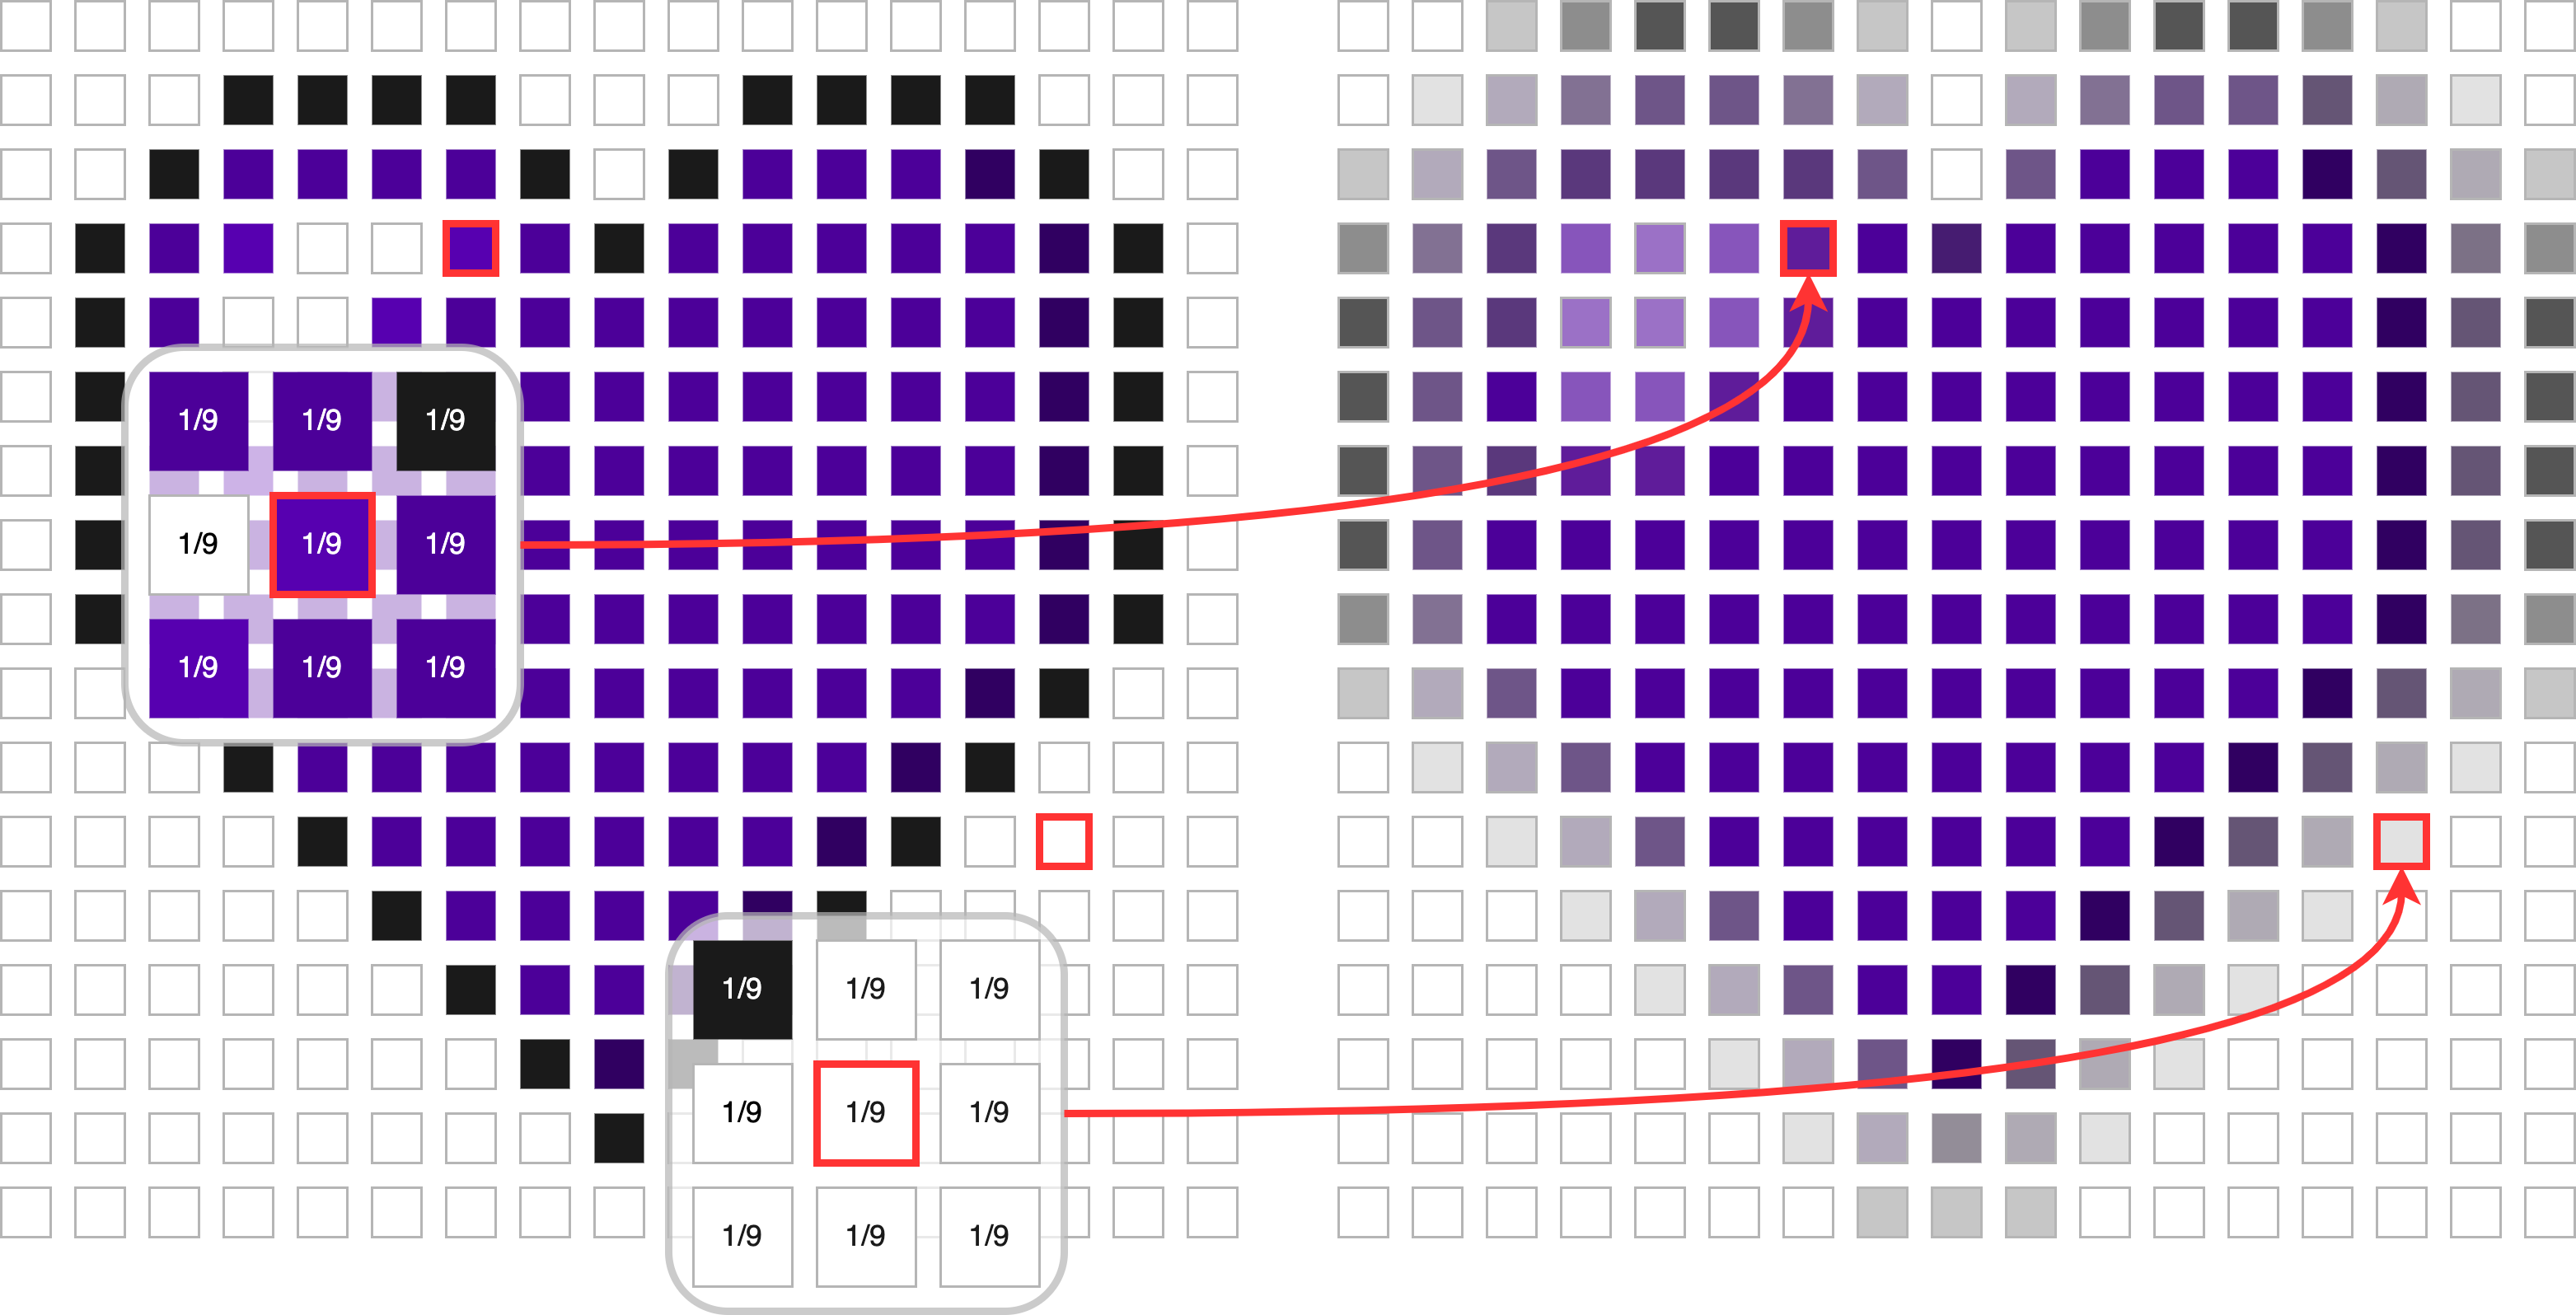
\includegraphics[width=0.9\textwidth]{figures/11/heart-convolution.png}
    \end{center}
    \caption{Floutage sur un voisinage de taille 9}
    \label{fig:floutage}
\end{figure}

\quessques Implémenter l'opération de floutage pour reproduire l'image \autoref{fig:img-blurry}. Attention à bien traiter les pixels du bord de l'image.
\ssques Changer la définition de voisinage en $ max(|x-i|, |y-j|) \leq 4 $ pour obtenir l'image \autoref{fig:img-very-blurry}.

\begin{figure}[h!]
    \centering
    \subfloat[Poivrons flous]{
        \label{fig:img-blurry}
        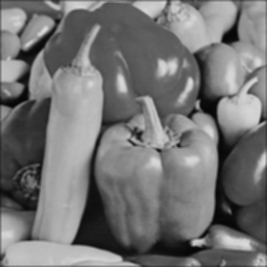
\includegraphics[width=0.45\textwidth]{figures/11/poivrons-blurry.png}
    }
    \subfloat[Poivrons très flous]{
        \label{fig:img-very-blurry}
        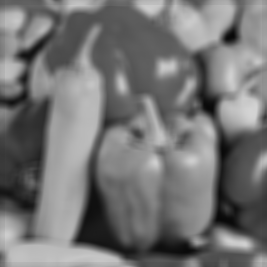
\includegraphics[width=0.45\textwidth]{figures/11/poivrons-very-blurry.png}
    }
    \caption{Transformation en flou}
\end{figure}

\subsection*{Détection de bords}

Une caractéristique de l'opération de floutage est qu'elle ne change pas beaucoup les zones "plates" où tous les pixels sont semblables, mais fait disparaître les bords. On peut considérer qu'une image $ M $ se décompose comme une superposition d'une image $ P $ qui est plate partout, et d'une image $ B $ ne contenant que les bords (c'est un peu comme quand un enfant dessine : d'abord les bords au crayon noir et ensuite la couleur), soit $ M = P + B $. Cette dernière égalité fait réellement intervenir des additions pixel par pixel, i.e. \[
    M[i, j] = P[i, j] + B[i, j]
\]
Alors la fonction $ \phi $ de floutage sélectionne seulement la partie plate : $ \phi(M) = P $. Mais alors on peut récupérer $ B $ ! Il suffit de faire la soustraction $ M - \phi(M) $.

\ques Utiliser les deux images générées à la question précédente pour extraire les images de bords et les visualiser en négatif comme \autoref{fig:edges}. Attention il faut gérer à la main le cas des pixels qui sortent de l'intervalle $ [0, 255] $.

\begin{figure}[h!]
    \begin{center}
        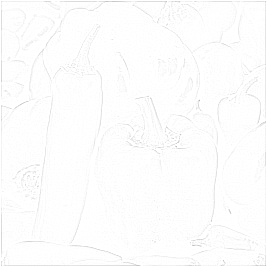
\includegraphics[width=0.45\textwidth]{figures/11/fine-edge-poivrons.png}
        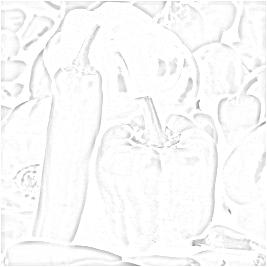
\includegraphics[width=0.45\textwidth]{figures/11/coarse-edge-poivrons.png}
    \end{center}
    \caption{Extraction des bords}
    \label{fig:edges}
\end{figure}


\section*{Représenter la couleur (hors-programme)}

Évidemment, la plupart des images ne sont pas en noir et blanc mais en couleur. Pour représenter un pixel d'une couleur, il ne faut plus un seul nombre mais 3, $ r $, $ g $ et $ b $, qui représentent respectivement le niveau de rouge, le niveau de vert et le niveau de bleu. À nouveau, chaque valeur évolue entre $ 0 $ et $ 255 $. Par exemple, un pixel de valeur \texttt{[0, 255, 255]} représente la couleur cyan (vert + bleu).

Si vous regardez de très près les pixels qui composent vos écrans d'ordinateur ou de téléphone, en utilisant une loupe ou bien en déposant une goutte d'eau sur l'écran, vous pourrez d'ailleurs voir des diodes rouges vertes et bleues, utilisées pour donner l'illusion de couleur.

Ainsi, une image en couleur est représentée par une matrice de pixels, où chaque pixel contient trois valeurs. Si l'image est de hauteur $ h $ et de largeur $ w $, sa matrice de représentation est donc de dimension $ h \times w \times 3 $.

Dans la suite on pourra utiliser les fonctions suivantes pour n'avoir à manipuler que des tableaux numpy:

\begin{minted}{python}
    def load_as_rgb_array(name):
        img = Image.open(name).convert('RGB')
        return np.asarray(img).copy()

    def save_rgb_array_as_img(array, name):
        img = Image.fromarray(array.astype(np.uint8), mode='RGB')
        img.save("{}.png".format(name), format='PNG')
\end{minted}

\quessques Quelle est la dimension de la matrice représentant une image $ 100 \times 100 $

\quessques Créer trois images \texttt{red.png}, \texttt{green.png} et \texttt{blue.png} de taille $ 100 \times 100 $ et représentant respectivement un carré rouge, un carré bleu et un carré vert.

\ssques Comment représenter le noir et le blanc dans les images en couleur ? Recréer l'image \autoref{fig:rgb-squares}, qui est de taille $ 100 \times 100 $.

\begin{figure}[h!]
    \begin{center}
        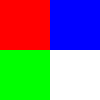
\includegraphics[width=0.4\textwidth]{figures/11/rgb-squares.png}
    \end{center}
    \caption{Les couleurs primaires et le blanc}
    \label{fig:rgb-squares}
\end{figure}

\ssques Quelle est la différence entre un pixel \texttt{[0, 0, 255]} et un pixel \texttt{[0, 0, 100]}.

\quessques Recréer l'image \autoref{fig:venn-couleur}, qui est de taille $ 100 \times 100 $ et où les cercles sont de diamètres $ 50 $ pixels.

\begin{figure}[h!]
    \begin{center}
        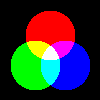
\includegraphics[width=0.4\textwidth]{figures/11/rgb-venn.png}
    \end{center}
    \caption{Diagramme de Venn des couleurs}
    \label{fig:venn-couleur}
\end{figure}

